\documentclass[border=4pt]{standalone}
\usepackage{tikz}
\usetikzlibrary{arrows.meta, positioning, calc, shapes.geometric, backgrounds, fit}
\usepackage{pgfplots}
\pgfplotsset{compat=1.18}
\usepgfplotslibrary{fillbetween}
\definecolor{deepblue}{RGB}{10, 40, 90}
\definecolor{spaceblue}{RGB}{30, 80, 160}
\definecolor{lightgray}{RGB}{245, 245, 248}
\definecolor{accentgold}{RGB}{180, 140, 40}
\definecolor{earthgreen}{RGB}{40, 120, 80}
\definecolor{warnred}{RGB}{170, 40, 40}
\begin{document}
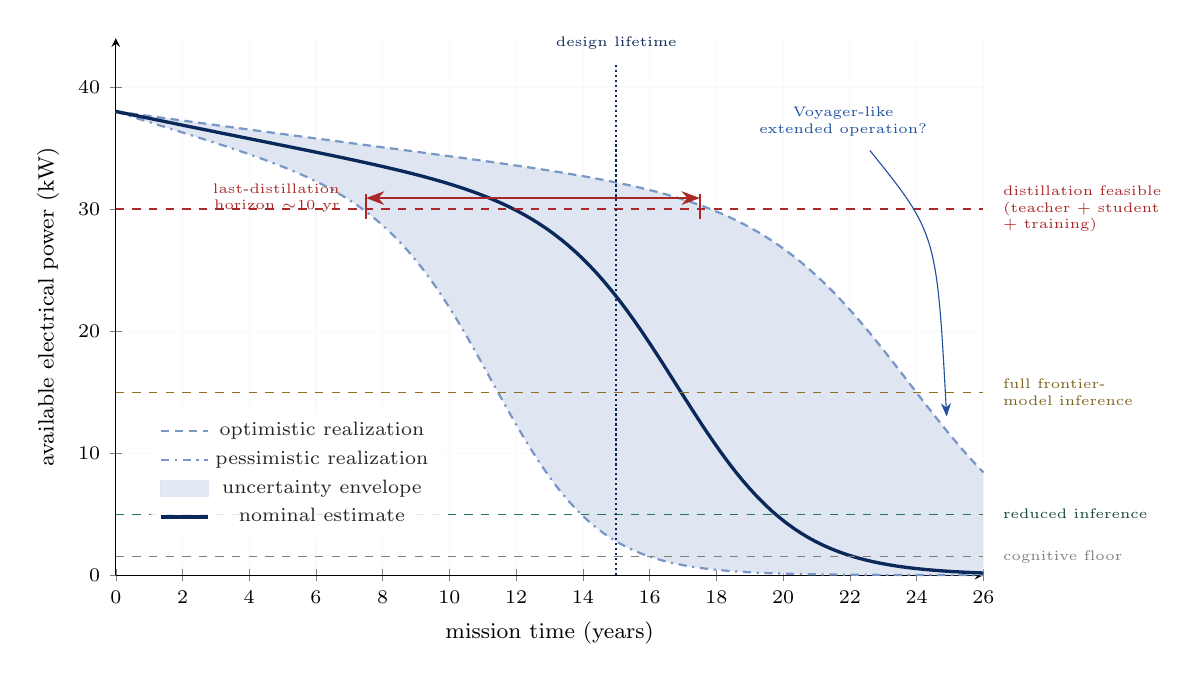
\begin{tikzpicture}
\begin{axis}[
  width=12.6cm, height=8.4cm,
  xlabel={mission time (years)}, ylabel={available electrical power (kW)},
  xmin=0, xmax=26, ymin=0, ymax=44,
  axis lines=left, grid=major, grid style={lightgray!60!white},
  tick label style={font=\scriptsize}, label style={font=\footnotesize},
  legend style={font=\scriptsize, at={(0.04,0.07)}, anchor=south west, draw=none, fill=white, fill opacity=0.85},
  clip=false
]
\addplot[name path=opt, spaceblue!60, thick, densely dashed, domain=0:26, samples=120]
  {38*exp(-0.010*x)/(1+exp((x-24)/2.2))};
\addplot[name path=pes, spaceblue!60, thick, dash dot, domain=0:26, samples=120]
  {38*exp(-0.022*x)/(1+exp((x-11.5)/1.6))};
\addplot[spaceblue!14] fill between[of=opt and pes];
\addplot[deepblue, very thick, domain=0:26, samples=120]
  {38*exp(-0.015*x)/(1+exp((x-17)/1.8))};
\legend{optimistic realization, pessimistic realization, uncertainty envelope, nominal estimate}

% thresholds, labels outside right edge
\addplot[warnred, dashed, domain=0:26] {30};
\node[font=\tiny, color=warnred, anchor=west, align=left] at (axis cs:26.3,30) {distillation feasible\\(teacher + student\\+ training)};
\addplot[accentgold!80!black, dashed, domain=0:26] {15};
\node[font=\tiny, color=accentgold!70!black, anchor=west, align=left] at (axis cs:26.3,15) {full frontier-\\model inference};
\addplot[earthgreen, dashed, domain=0:26] {5};
\node[font=\tiny, color=earthgreen!60!black, anchor=west] at (axis cs:26.3,5) {reduced inference};
\addplot[gray, dashed, domain=0:26] {1.5};
\node[font=\tiny, color=gray, anchor=west] at (axis cs:26.3,1.5) {cognitive floor};

% design lifetime
\draw[densely dotted, thick, deepblue] (axis cs:15,0) -- (axis cs:15,42);
\node[font=\tiny, color=deepblue, anchor=south] at (axis cs:15,42.3) {design lifetime};

% horizon-uncertainty: ticks at pes/opt crossings of 30 kW, arrow just above the line
\draw[warnred, thick] (axis cs:7.5,29.2) -- (axis cs:7.5,31.2);
\draw[warnred, thick] (axis cs:17.5,29.2) -- (axis cs:17.5,31.2);
\draw[{Stealth}-{Stealth}, warnred, thick] (axis cs:7.5,30.9) -- (axis cs:17.5,30.9);
\node[font=\tiny, color=warnred, anchor=east, align=right] at (axis cs:7.0,30.9) {last-distillation\\horizon $\sim$10 yr};

% Voyager note in empty upper-right, arrow to optimistic tail
\node[font=\tiny, color=spaceblue, align=center, anchor=south] (voy) at (axis cs:21.8,35.2) {Voyager-like\\extended operation?};
\draw[-{Stealth}, spaceblue, thin] (axis cs:22.6,34.8) .. controls (axis cs:24.6,28) .. (axis cs:24.9,13.0);
\end{axis}
\end{tikzpicture}
\end{document}
